
\section{Methodologies}
\label{sec5_3}

This section discusses the design of the processing pipeline and details the principles of the consisting modules.
Before the actual centerline extraction begins, several processing aims to removing noises and smoothing the irregular surfaces need to be run to guarantee the quality of the input surface.
The image-based surface model of the blood vessels needs series of postprocessing steps depicted in Fig. \ref{fig:DataFlow5} to meet the requirements of the centerline computing module. %
Among these processing steps, the first one is the validation of the connectivity of the consisting polygons.
During this process, the largest possible connected regions of the surface model are extracted.
Next, the surface smoothing step is needed to depress the ``crusts" and ``stairs" in the surface.
Then the normal vectors (i.e., normals) are computed to mark the ``inside" and the ``outside" of the surface model.
After that, the consisting polygons need to be subdivided under a specified criterion to facilitate the computation of the centerline extraction at the cost of longer computation time. %

%\subsection{Processing on Image-Based Surface Model}

\subsection{Connectivity Validation and Largest Region Extraction}

In this paper, the vasculature surface model is generated from the original medical volumetric data set by applying the approaches reported in our previous work \cite{Yang2014ICRA}. %
In order to find the largest region spanning the surface of the vasculature, the connectivity among the vertices in the image-based surface model needs to be thoroughly validated at the beginning of the processing. %
The inner working is to extract consisting polygons that share common vertices and meet some requirements.
In the present paper we implement the algorithm to extract the largest connected region from the input surface.
\begin{figure}[t]
\centering
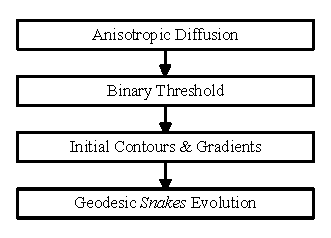
\includegraphics[width=3.2in]{figures/chap05/DataFlow.eps}
\caption{Overview of the work flow.}
\label{fig:DataFlow5}
\end{figure}

\subsection{Surface Smoothing and Normals Computing}

There are plenty of methods used for the surfaces smoothing in visualization.
To overcome the ``facets" by-produced during this approximation, an optimal surface smoothing algorithm treating this problem as low-pass filtering by extending Fourier analysis is adopted \cite{Taubin1996}. %
The adopted method is built upon the formulation of the \emph{discrete graph signals}, which means the functions based on directed graph.
The directed graph $G$ represents the polyhedral surfaces in this problem, which is denoted as the set $\left\{ 1, \ldots, n \right\}$ of nodes with a set of neighborhoods $\left\{ i^{\ast}: i = 1, \ldots, n \right\}$ of node $i$. %
A discrete graph signal can be represented as a vector $x = \left[ x_1, \ldots, x_n \right]^T$, where each component of the vector corresponds one node of the graph.
A polyhedral surface $S = \{ V, F \}$ of $n$ vertices can be treated as a directed graph, where the vertices $V$ corresponds the set of nodes $n$ and the faces $F$ the polygons formed by connected nodes. %

The discrete surface signal, the discrete graph signal defined on the associated graph, can be visualized as a piece-wise linear function defined on the surface.
The computation of the Discrete Fourier Transform (DFT) of the discrete surface signal defined on the surface is achieved by decomposing the surface signals as a linear combination of the eigenvectors of the Laplacian: %
\begin{equation}
\label{eqn:Laplacian}
\Delta x_i = \sum_{j \in i^{\ast}} w_{ij} \left( x_j - x_i \right),
\end{equation}
where $w_{ij}$ is the positive weight for each difference of $x_j - x_i$ and for a given vertex $i$, the sum of its weights are always one.
The matrix form of (\ref{eqn:Laplacian}) is
\begin{equation}
\label{eqn:LaplacianMatrix}
\Delta x = - K x,
\end{equation}
where $K = I - W$, with $I$ an identity matrix and $W$ the matrix of weights $w_{ij}$.

Choosing $0 \leq k_1 \leq \ldots \leq k_n \leq 2 $ as the eigenvalues of $K$, $r_1, \ldots, r_n$ the corresponding right eigenvectors, and $d_1, \ldots, d_n$ the associated dual basis of these eigenvectors, the above $K$ can be obtained as $K = \sum_{i} k_i r_i d_i^T$. %
%\begin{equation}
%\label{eqn:K}
%K = \sum_{i} k_i r_i d_i^T.
%\end{equation}
Thus there is a unique decomposition the discrete graph signal $x$, which can be obtained as a linear combination of the right eigenvectors $x = \sum_{i} \hat{x}_i r_i$, %$r_1, \ldots, r_n$
%\begin{equation}
%\label{eqn:x}
%x = \sum_{i} \hat{x}_i r_i,
%\end{equation}
where $\hat{x}_i = d_i^T x$ is the DFT of $x$.

According to signal processing theory, the filtering calculation on the signal $x$ is to change its frequency distribution at the reference of a transfer function $f$:
\begin{equation}
\bar{x} = \sum_{i} f(k_i) \hat{x}_i r_i = \left( \sum_{i} f(k_i) r_i d_i^T \right) x.
\end{equation}
The \emph{low-pass filtering} mechanism can be implemented by adjusting the weights in the following polynomial approximation
\begin{equation}
\label{eqn:Approximation}
f_{N}(k) = w_0 \frac{\theta}{\pi} T_0 (1 - k / 2) + w_n \sum_{n} \frac{2 \sin (n \theta)}{n \pi} T_n(1 - k / 2),
\end{equation}
where $\theta$ is the unique solution of $k = 2 (1 - \cos \theta)$ on $[0, \pi / 2]$, and $T$ the Chebyshev polynomial.
Here in this paper, the weights in (\ref{eqn:Approximation}) is adjusted to form a Hamming window, among sorts of them, which is demonstrated as follows:
\begin{equation}
\label{eqn:HammingWindow}
w_n = 0.54 + 0.46 \cos (n \pi / (N + 1) ).
\end{equation}

The normal vectors to the surfaces are computed after the surfaces are smoothed.

\subsection{Surface Subdivision}

A modified butterfly scheme for surface subdivision is used in order to refine the smoothed surface model \cite{Zorin1996}.
This scheme is designed in the flavor of interpolating and has been proved to be useful in the circumstances of subdivision for the complex especially irregular surfaces.
The ultimate goal is to improve the visualization of the input surface model without affecting its original shape.
The scalar value associated with the new vertex of the 2-dimensional triangulation is generated by calculating weighted sum of neighboring vertices using the proposed interpolation scheme. %
These vertices located in the neighborhood form the subdivision stencil, which determines the features of the scheme.
By analyzing the stencil, the scheme can quickly identify the relationship between the new vertex and the topology of its neighborhood.
The two most important cases in the surface are the regular sites and the extraordinary sites.
Once the initial subdivision cycles completed, the largest number of the vertices possessing the valence other than six is not exceeding one.
The new scalar value for the midpoint on each edge of the triangulation is calculated by the subdivision scheme falls into the following cases:
(1) edge connects two regular vertices;
(2) edge connects an extraordinary vertex and a regular vertex;
(3) edge connects two extraordinary vertices; and
(4) boundary edges.
%\begin{itemize}
%\item edge connects two regular vertices;
%\item edge connects an extraordinary vertex and a regular vertex;
%\item edge connects two extraordinary vertices;
%\item boundary edges.
%\end{itemize}
Among the above cases, only the first one belongs to the regular case, whilst the rest belong to the extraordinary case.

\subsection{Centerlines Extraction}

Centerlines, or medial axis, can be generally defined as the loci of the centers of the maximal inscribed disks (in 2D space) or spheres (in 3D space) inside an object.
Conversely, the envelop of all maximal inscribed disks/spheres is the boundary/surface of the object that contains these disks/spheres \cite{Amenta2001}.
Our approach employed the method demonstrated in \cite{Antiga2003}, which treats the centerlines as the minimal action paths on the Voronoi diagrams inside the model surface.
The Voronoi diagrams are the discrete approximation of the medial axis of the shape in two or three dimensional space.
The minimization of the line integral of the action path, which links two vertices in the Voronoi diagram, generates the center points that locally maximize their minimal distances to the boundary of the surface.
To do this, the method firstly computes the following Eikonal equation from a given starting point located on the Voronoi diagram
\begin{equation}
\label{eqn:Voronoi}
\left| \nabla T \right| = \frac{1}{R(u)},
\end{equation}
where $T$ marks the time of arrival, $R$ the radius of the maximal inscribed sphere at the time $T$, and $u$ the parametric space of the Voronoi diagram.
Then the centerline is obtained by calculating the following equation upon the previously demonstrated computation terminated:
\begin{equation}
\label{eqn:Centerlines}
\frac{dc}{ds} = - \nabla T,
\end{equation}
where $c$ denotes the centerlines, and $s$ the parametric space of $c$.
As a matter of fact, computation illustrated by (\ref{eqn:Centerlines}) is equivalent to finding the resulting centerline by applying the steepest descent method at each point on the Voronoi diagram. 